% Chapter 4

\chapter{Applying Convolutional Neural Networks} % Main chapter title

\label{Chapter4}

%-------------------------------------------------------------------------------
%-------------------------------------------------------------------------------

\section{Creating the Dataset}

Creating an annotated dataset is often the longest and most tedious part of any machine learning task. A common complaint against deep learning is that you need large amounts of data to train properly generalized model. This can be mitigated somewhat through transfer learning, but for good generalization of a network sufficient training data is needed. The goal for our network is that it will be effective on other areas outside our main site of BFREE which might have variations in lighting conditions, pixel resolution, etc.. Our dataset can be found at DATASET-URL-INSERT-HERE.

\begin{figure}[ht]
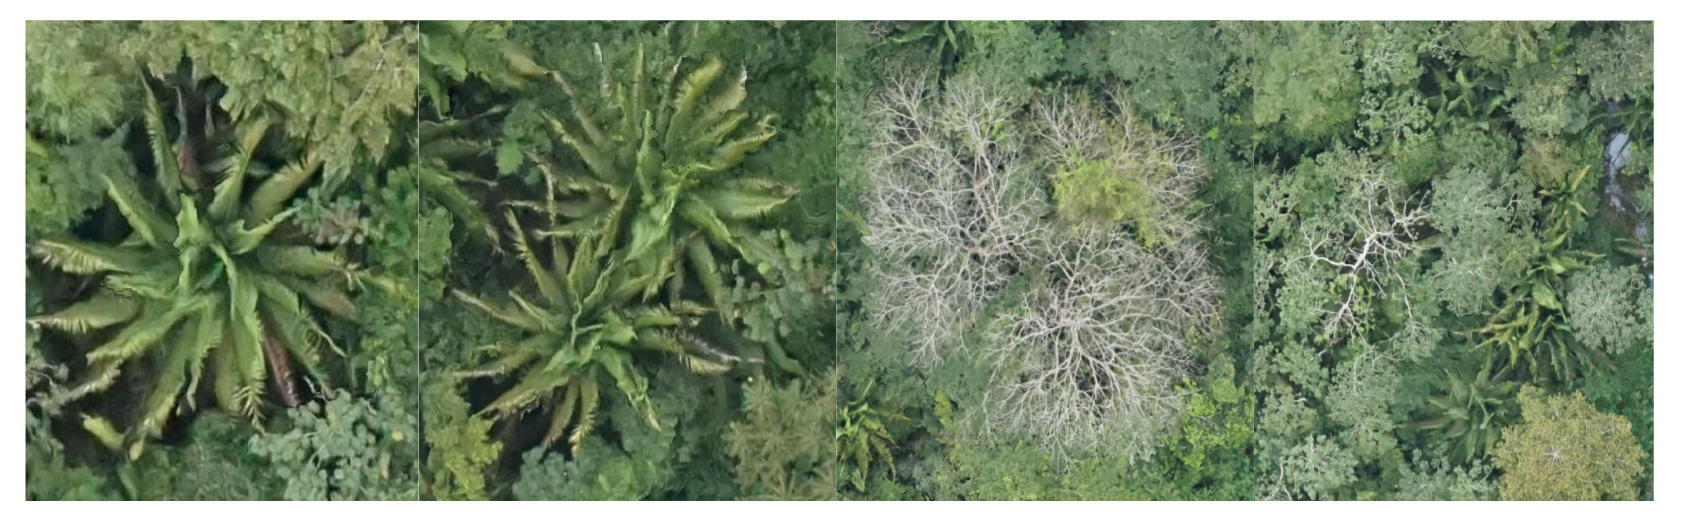
\includegraphics[width=1.0\textwidth]{Figures/Palm-Deciduous.png}
\caption{Example Instances of Cohune Palm Trees and Deciduous Trees from our dataset.}
\label{fig:Palm-Deciduous}
\end{figure}

\subsection{Labeling Tool}

In order to parallelize the labeling process we developed a simple web tool for decentralizing the task of labeling images. The web tool was a built using a mix of javascript and python; django was used to run the server and store data, openstreetmap was used for displaying the image and drawing boxes, and leaflet for working with GIS data. The web tool was run on a local server that allowed users to log on remotely and label data at their convenience. ~\ref{fig:LabelingTool} shows an example of using the tool. Users were given tiles cropped from the orthomosaic. Each tile corresponds to approximately $100m^2$ of rainforest. In order to help keep the labeling consistent a demo video was shown to volunteers that described how to label a tile. Each tile annotation contains a list of bounding boxes with a corresponding class label; either Cohune palm or deciduous. The data was stored on the server in a database and served as a CSV on request.

\begin{figure}[ht]
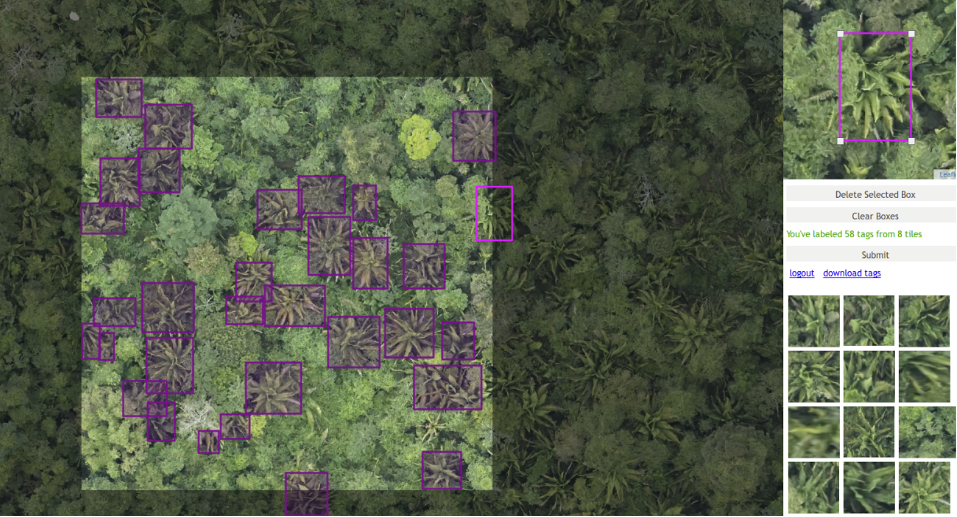
\includegraphics[width=1.0\textwidth]{Figures/LabelingTool.png}
\caption{Labeling tool in action. Note that you are shown surrounding area of the tile allowing the user to label palm trees that overlap two segments. Thumbnails on the lower right allow easy visual grepping of currently labeled trees}
\label{fig:LabelingTool}
\end{figure}

\subsection{Labeling Noise}

Our volunteers came from a mix of ecology students at the University of North Carolina Wilmington who labeled Cohune Palm trees and computer science students at University of California San Diego who labeled Deciduous Trees. Between labelers we found considerable variation in accuracy and annotation styles.

First we noticed that many tiles had obviously missing bounding boxes. We hypothesize that this is due to labeler fatigue. The tiles we present are quite dense with trees and are a very uniform green. The author noticed in his own labeling that over time it became harder to focus and be consistent with labeling. This could be mitigated in the future by presenting smaller tiles and limiting the amount of time users are allowed to label at one time.

Secondly we saw that bounding boxes with respect to crowding i.e. overlapping trees as well as occluded trees had a large variation. Some users created one box per crowd while some were meticulous in labeling each tree. Some users labeled tiny portions of heavily occluded palm trees while others skipped even partially occluded trees. One thought for future work would be to present users with examples for each scenario and then present tests which are used to evaluate the labelers skill.

In order to combat this label noise the author went through the dataset and cleaned up bounding boxes with respect to crowded or occluded trees and added missing annotation to each tile. This led to significantly lower average loss and higher evaluation metrics.

\subsection{Dataset Statistics} \label{section:statistics}

In order to get a better understanding of the dataset we examine the position of each bounding box in the image frame as well as the distribution of the square root of bounding boxes areas. The latter is very import as its informative for choosing bounding box priors for the network. Notice that the distribution for each class is roughly Gaussian centered around mean $210 pixels^2$ for Cohune Palms and $130 pixels^2$ for Deciduous trees. Deciduous trees by inspection have a much higher standard deviation then Cohune Palms with more outliers. Also note that we have a heavy class imbalance with approximately 10x Cohune Palm Trees when compared to Deciduous Trees. This will be addressed in ~\ref{section:class_imbalance}.

\begin{figure}[ht]
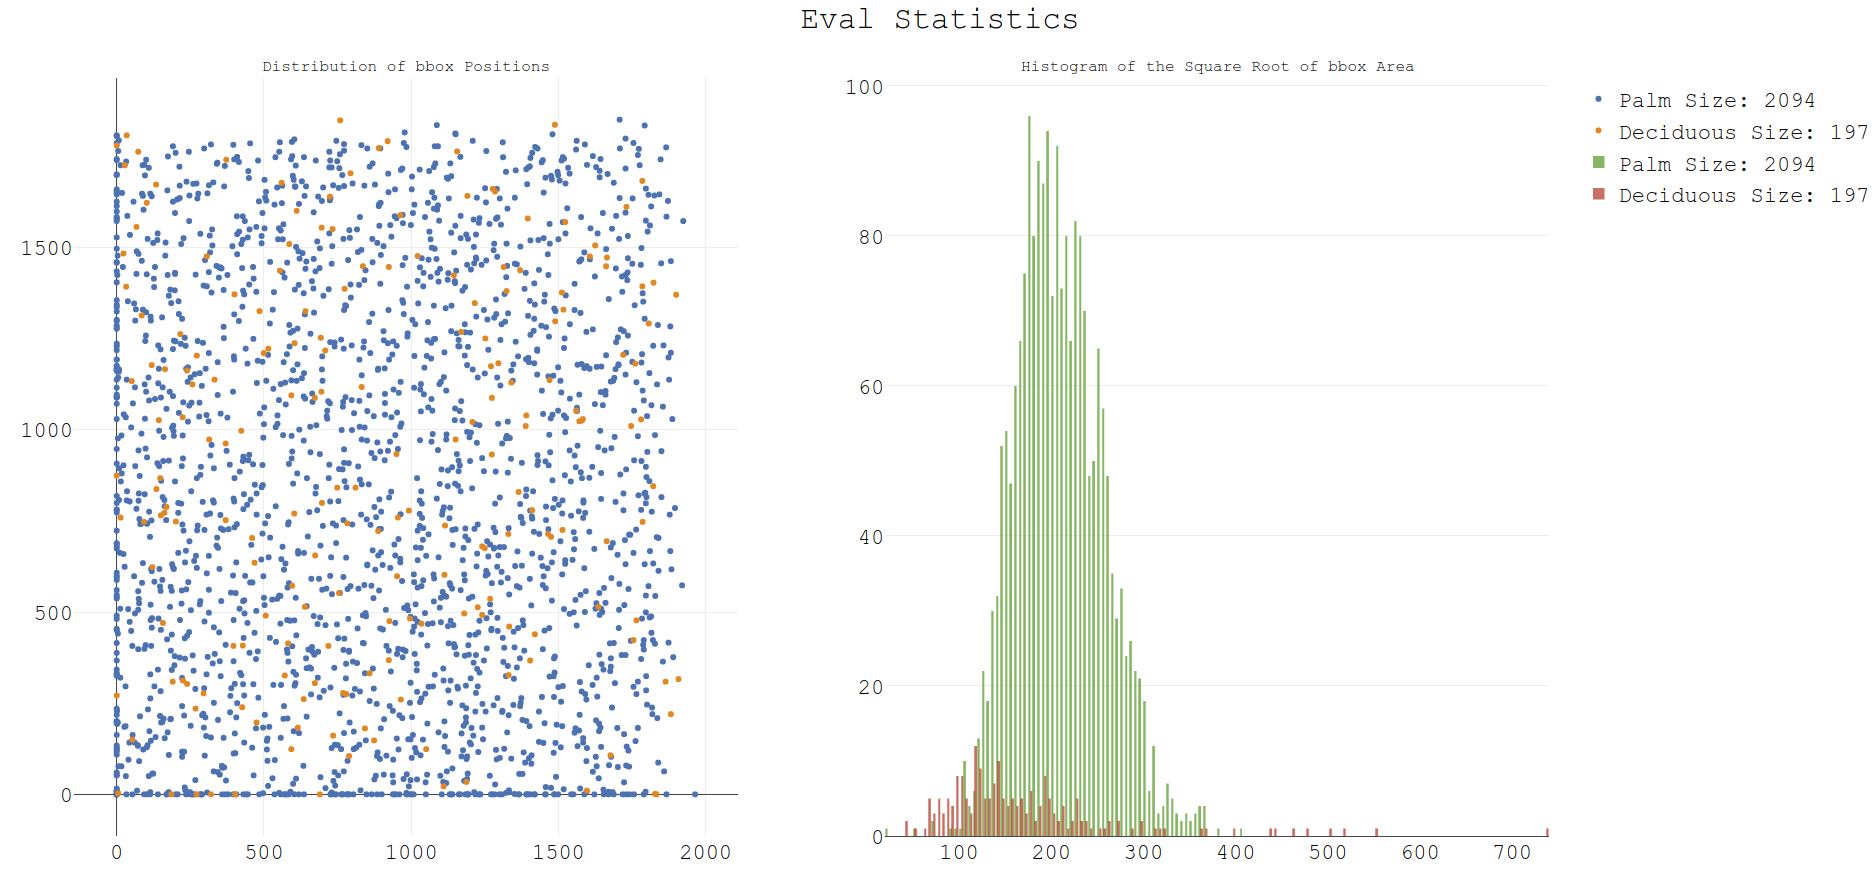
\includegraphics[width=1.0\textwidth]{Figures/EvalStats.png}
\caption{Bounding Box Statistics from the Evaluation set.}
\label{fig:EvalStats}
\end{figure}

\begin{figure}[ht]
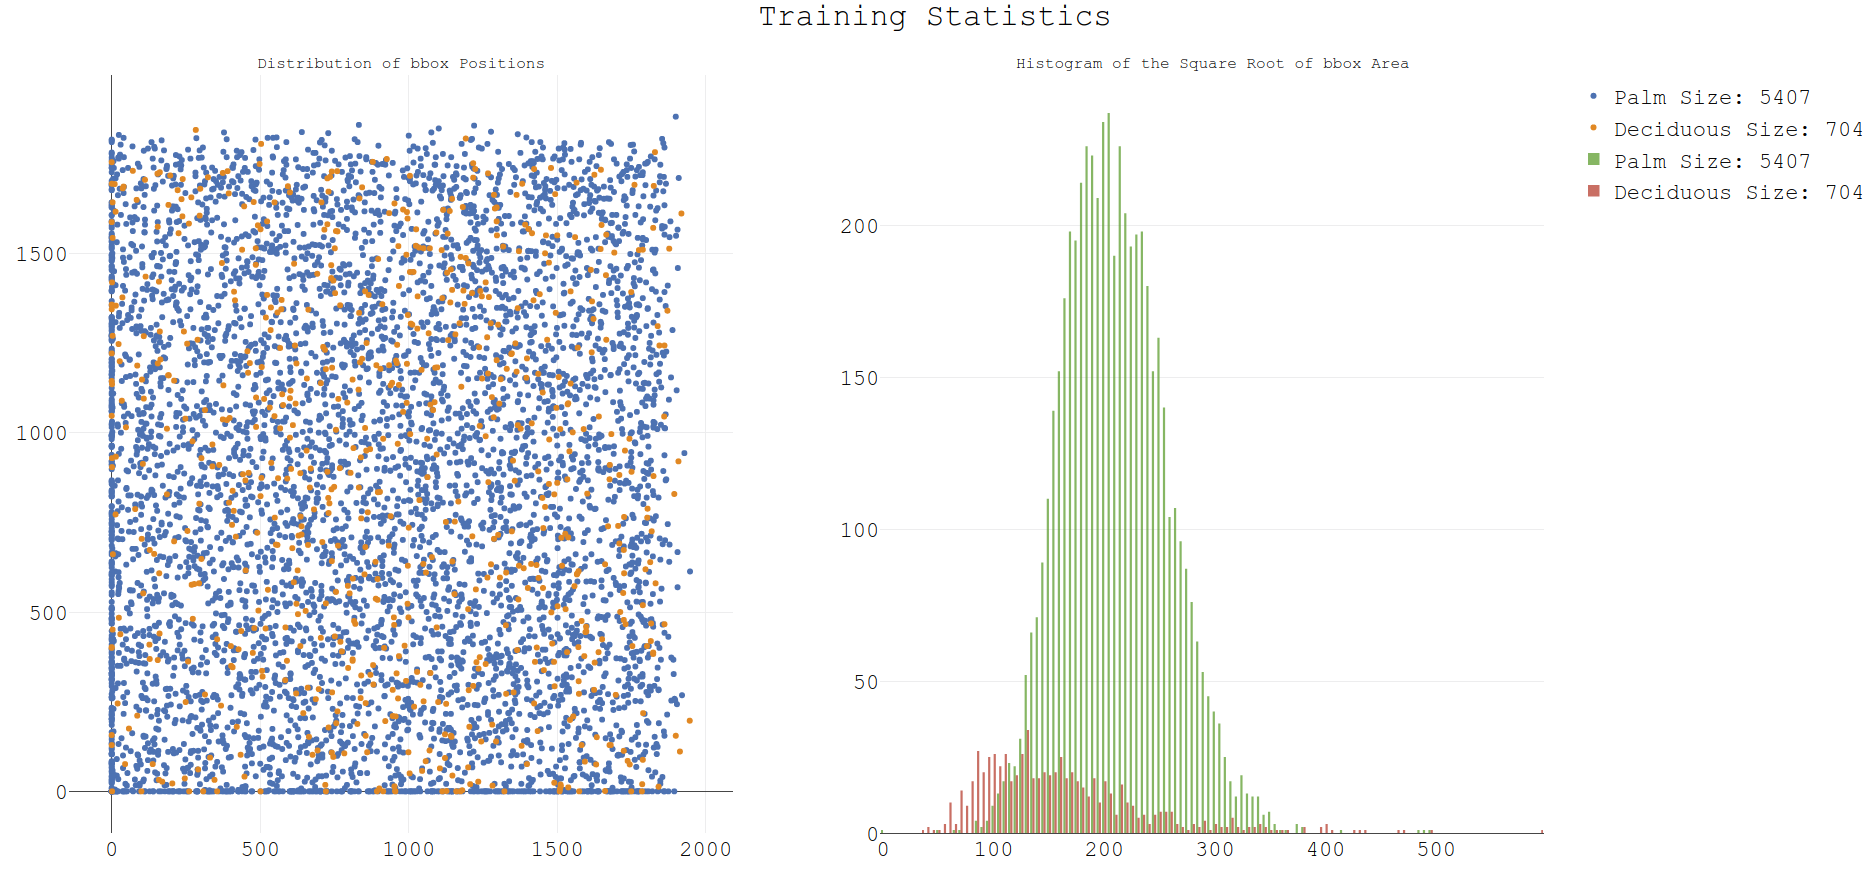
\includegraphics[width=1.0\textwidth]{Figures/TrainingStats.png}
\caption{Bounding Box Statistics from the Training set.}
\label{fig:TrainingStats}
\end{figure}

\section{Training the Network}

The dataset we present is still relatively small compared to many used to train deep neural networks from scratch. We compensate by using a pretrained network. YOLOv2 comes with several pretrained networks on the common classification datasets ImageNet and object detection datasets COCO \cite{COCO}, Pascal VOC \cite{VOC}.

The main difference between the pretrained networks is that the ImageNet weights do not include the final convolution layer which is used for regression while the other two pretrained networks do. We found that training with the ImageNet base network led to better performance. We hypothesize that this is because the other networks have already over fit the regression task to the bounding box shapes and classes in the object detection datasets.

We trained our networks using NVIDIA GTX 1080 graphics card, Intel Core i7 7th gen, and 32GB of RAM. The full desktop setup cost was under $\$3000$. On average we trained for approximately 20,000 iterations on our dataset with a batch size of 32 taking roughly 18 hours. We used a simple learning rate schedule that started at 0.001 and dropped by 10x every 7,500 iterations. This is a fairly short training regime when compared to training on a dataset which may contain upwards of a million images like ImageNet.

\begin{table}[]
\centering
\caption{My caption}\label{table:DesktopBOM}
\begin{tabular}{ll}
item                & cost       \\ \hline
Noctua NH-L12       & \$60.00    \\
NVIDIA GTX 1080     & \$700.00   \\
Silverstone ML07    & \$70.00    \\
Corsair SF 600W     & \$120.00   \\
Samsung 850 EVO 1TB & \$350.00   \\ \hline
Total               & \$1,970.00 \\
\end{tabular}
\end{table}


\subsection{Network Resolution}

YOLOv2 takes advantage of its ability to have dynamically resized inputs in training by randomly resizing the network input every 10 iterations. This has the effect of training on various resolutions of data making the algorithm more robust to variance in resolution at run time; an important step to generalizing our network to images with lower resolution. We limit the resize to three strides above and below our desired input resolution i.e. if our desired inference resolution is 416 then the lower limit on training would be 320 and the maximum would be 512. We experiment with three different resolutions, 416, 608, 800 and show the performance of each at ~\ref{section:results}.

\subsection{Class Imbalance}\label{section:class_imbalance}

Our dataset suffers from a large class imbalance between Cohune Palm Trees and Deciduous trees as shown in ~\ref{fig:TrainingStats}.

\section{Evaluating the Network}

Evaluating the performance of the network for an object detector is much less straight forward then for a classification network. We not only have to classify an object but we need to judge how well the generated bounding boxes match the ground truth; all the while trying to minimize the number of false positives that are produced. With the number of variables being juggled different interpretations arise for what a \textit{good} network performance looks like. A commonly accepted metric used by \cite{COCO} is Average Precision (AP) which is a single value that attempts to capture a coherent metric of precision. While others might display performance as the relationship between probability of detection vs probability of false alarm. In the next paragraph I will cover the basics of evaluating detections and the metrics we adopt for this work.

Detections generated by the network for an image fall into three categories: True Positive (TP), False Positive (FP), and False Negative (FN). In order to classify a detection as TP, FP, or FN we define Intersection over Union (IoU) between a network generated bounding box and a human bounding box as $IoU = \frac{Intersection of Boxes}{Overlap of Boxes}$. See ~\ref{fig:IOU} for an example of IoU. Given network detections and human labels for an image we can define TP as a network detection and human label with an IoU greater than a certain threshold and a matching class. Both the Pascal VOC and COCO datasets evaluate results using an IoU of $50\%$ and we adopt this standard. Furthermore there can only be a single TP per ground truth. If there are more than one network detection that meet the criteria for TP the detection with max IoU is accepted and the rest are considered as FPs. FPs are all network detections that do not have a corresponding ground truth. FN are all human labels that do not have a corresponding network detection. Now we can define $precision = \frac{TP}{TP+FP}$ and $recall = \frac{TP}{TP + FN}$ as the two metrics we will use to evaluate performance. Precision gives a sense of how relevant the returned detections are i.e. high precision corresponds to returning mainly good detections with few false positives. While recall represents the percentage of human labels correctly returned.

Each network detection has an associated confidence in how likely it thinks there is an object of that class present at that location. In order to calculate Average Precision we divide our confidence threshold from $0$ to $1$ with steps of size $0.01$. We then calculate precision at each step in our confidence range excluding any detection that have a confidence below that threshold which are then averaged to find AP. Another common way to represent network performance are precision recall graphs. We calculate recall at each confidence threshold like before and then simply plot the precision and recall as a pair. The desired shape for a PR curve is a knee which shows that precision remains high as recall increases and confidence threshold decreases.

We use pycoco api open source evaluation tools \cite{COCO} to keep our results consistent with state of the art object detection evaluation metrics. This also means our dataset is in the COCO format and can thus be trained on any open source object detector that uses that format for training and evaluation.

\begin{figure}[ht]
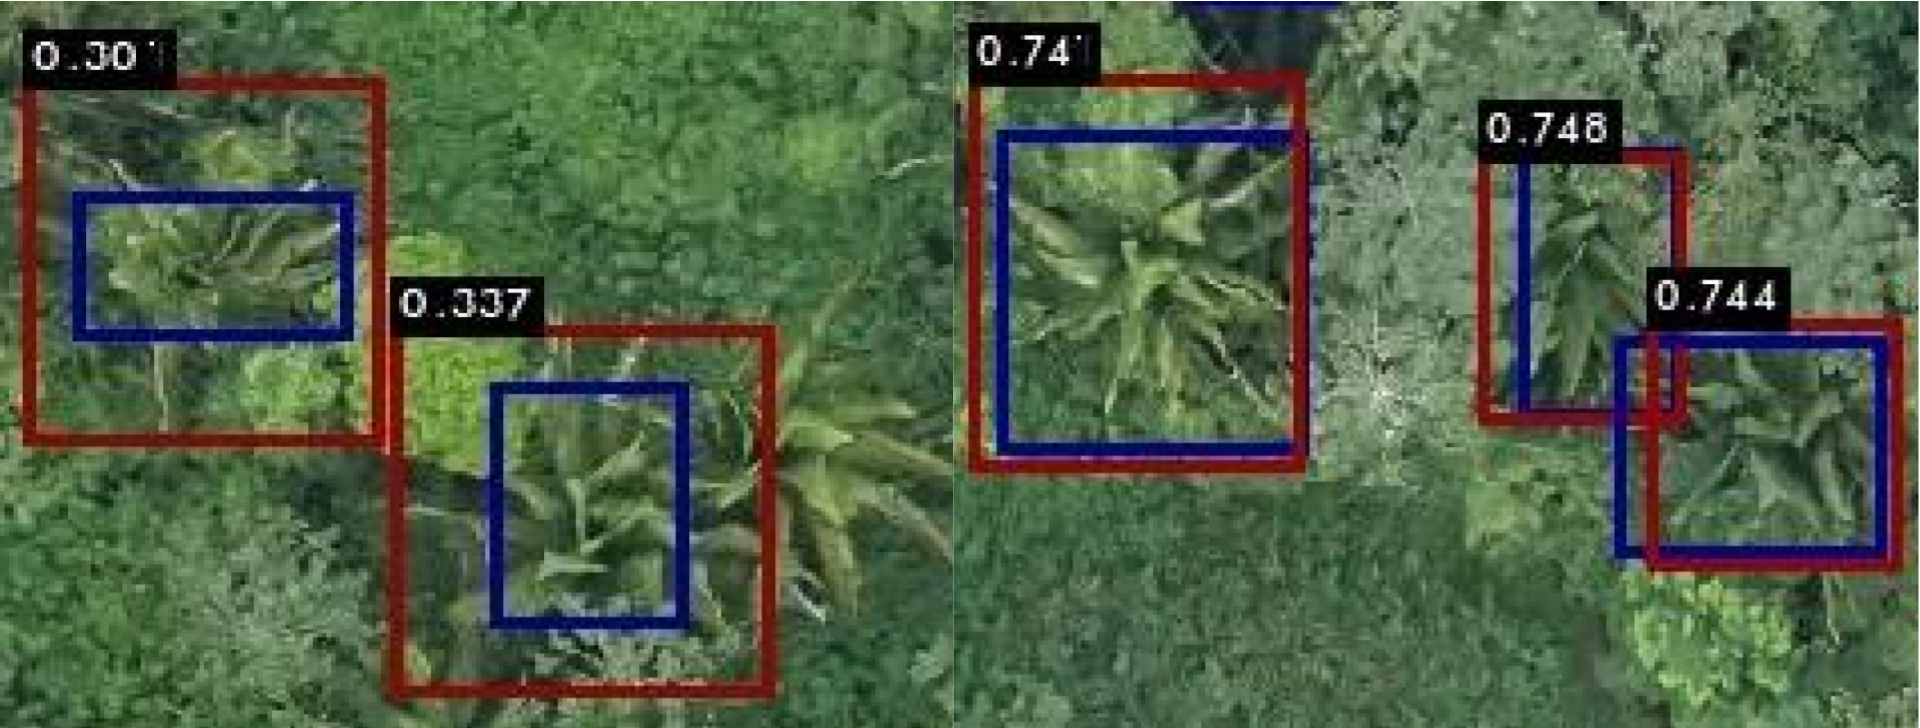
\includegraphics[width=1.0\textwidth]{Figures/IOU.png}
\caption{Example of IOU scores where blue corresponds to the human box and red corresponds to network detections.}
\label{fig:IOU}
\end{figure}
